\section{Implementation}

The following section outlines the key steps for capturing
depth images, converting them into point clouds and using these point clouds
for 3D reconstruction.

\subsection{Capturing Clouds and Background Subtraction}

In order to align the different point clouds, it is necessary to helpful to remove
noise and outliers. The room, floor, and other features
(like your arm holding the camera) are not relevant when scanning a particular object.

A sophisticated approach might adopt a technique for \textit{background subtraction}. \cite{piccardi2004background} surveys a few methods such as  taking an ``empty'' snapshot and subtracting it from subsequent ones to isolate the model.
Advanced approaches maintain models of the background to accomodate for change over time and so on.
For our purpose of capturing toy examples, it (mostly) suffices to set a maximum depth
and discard the back wall of a fixed scene.

\begin{figure}[h]
\centering
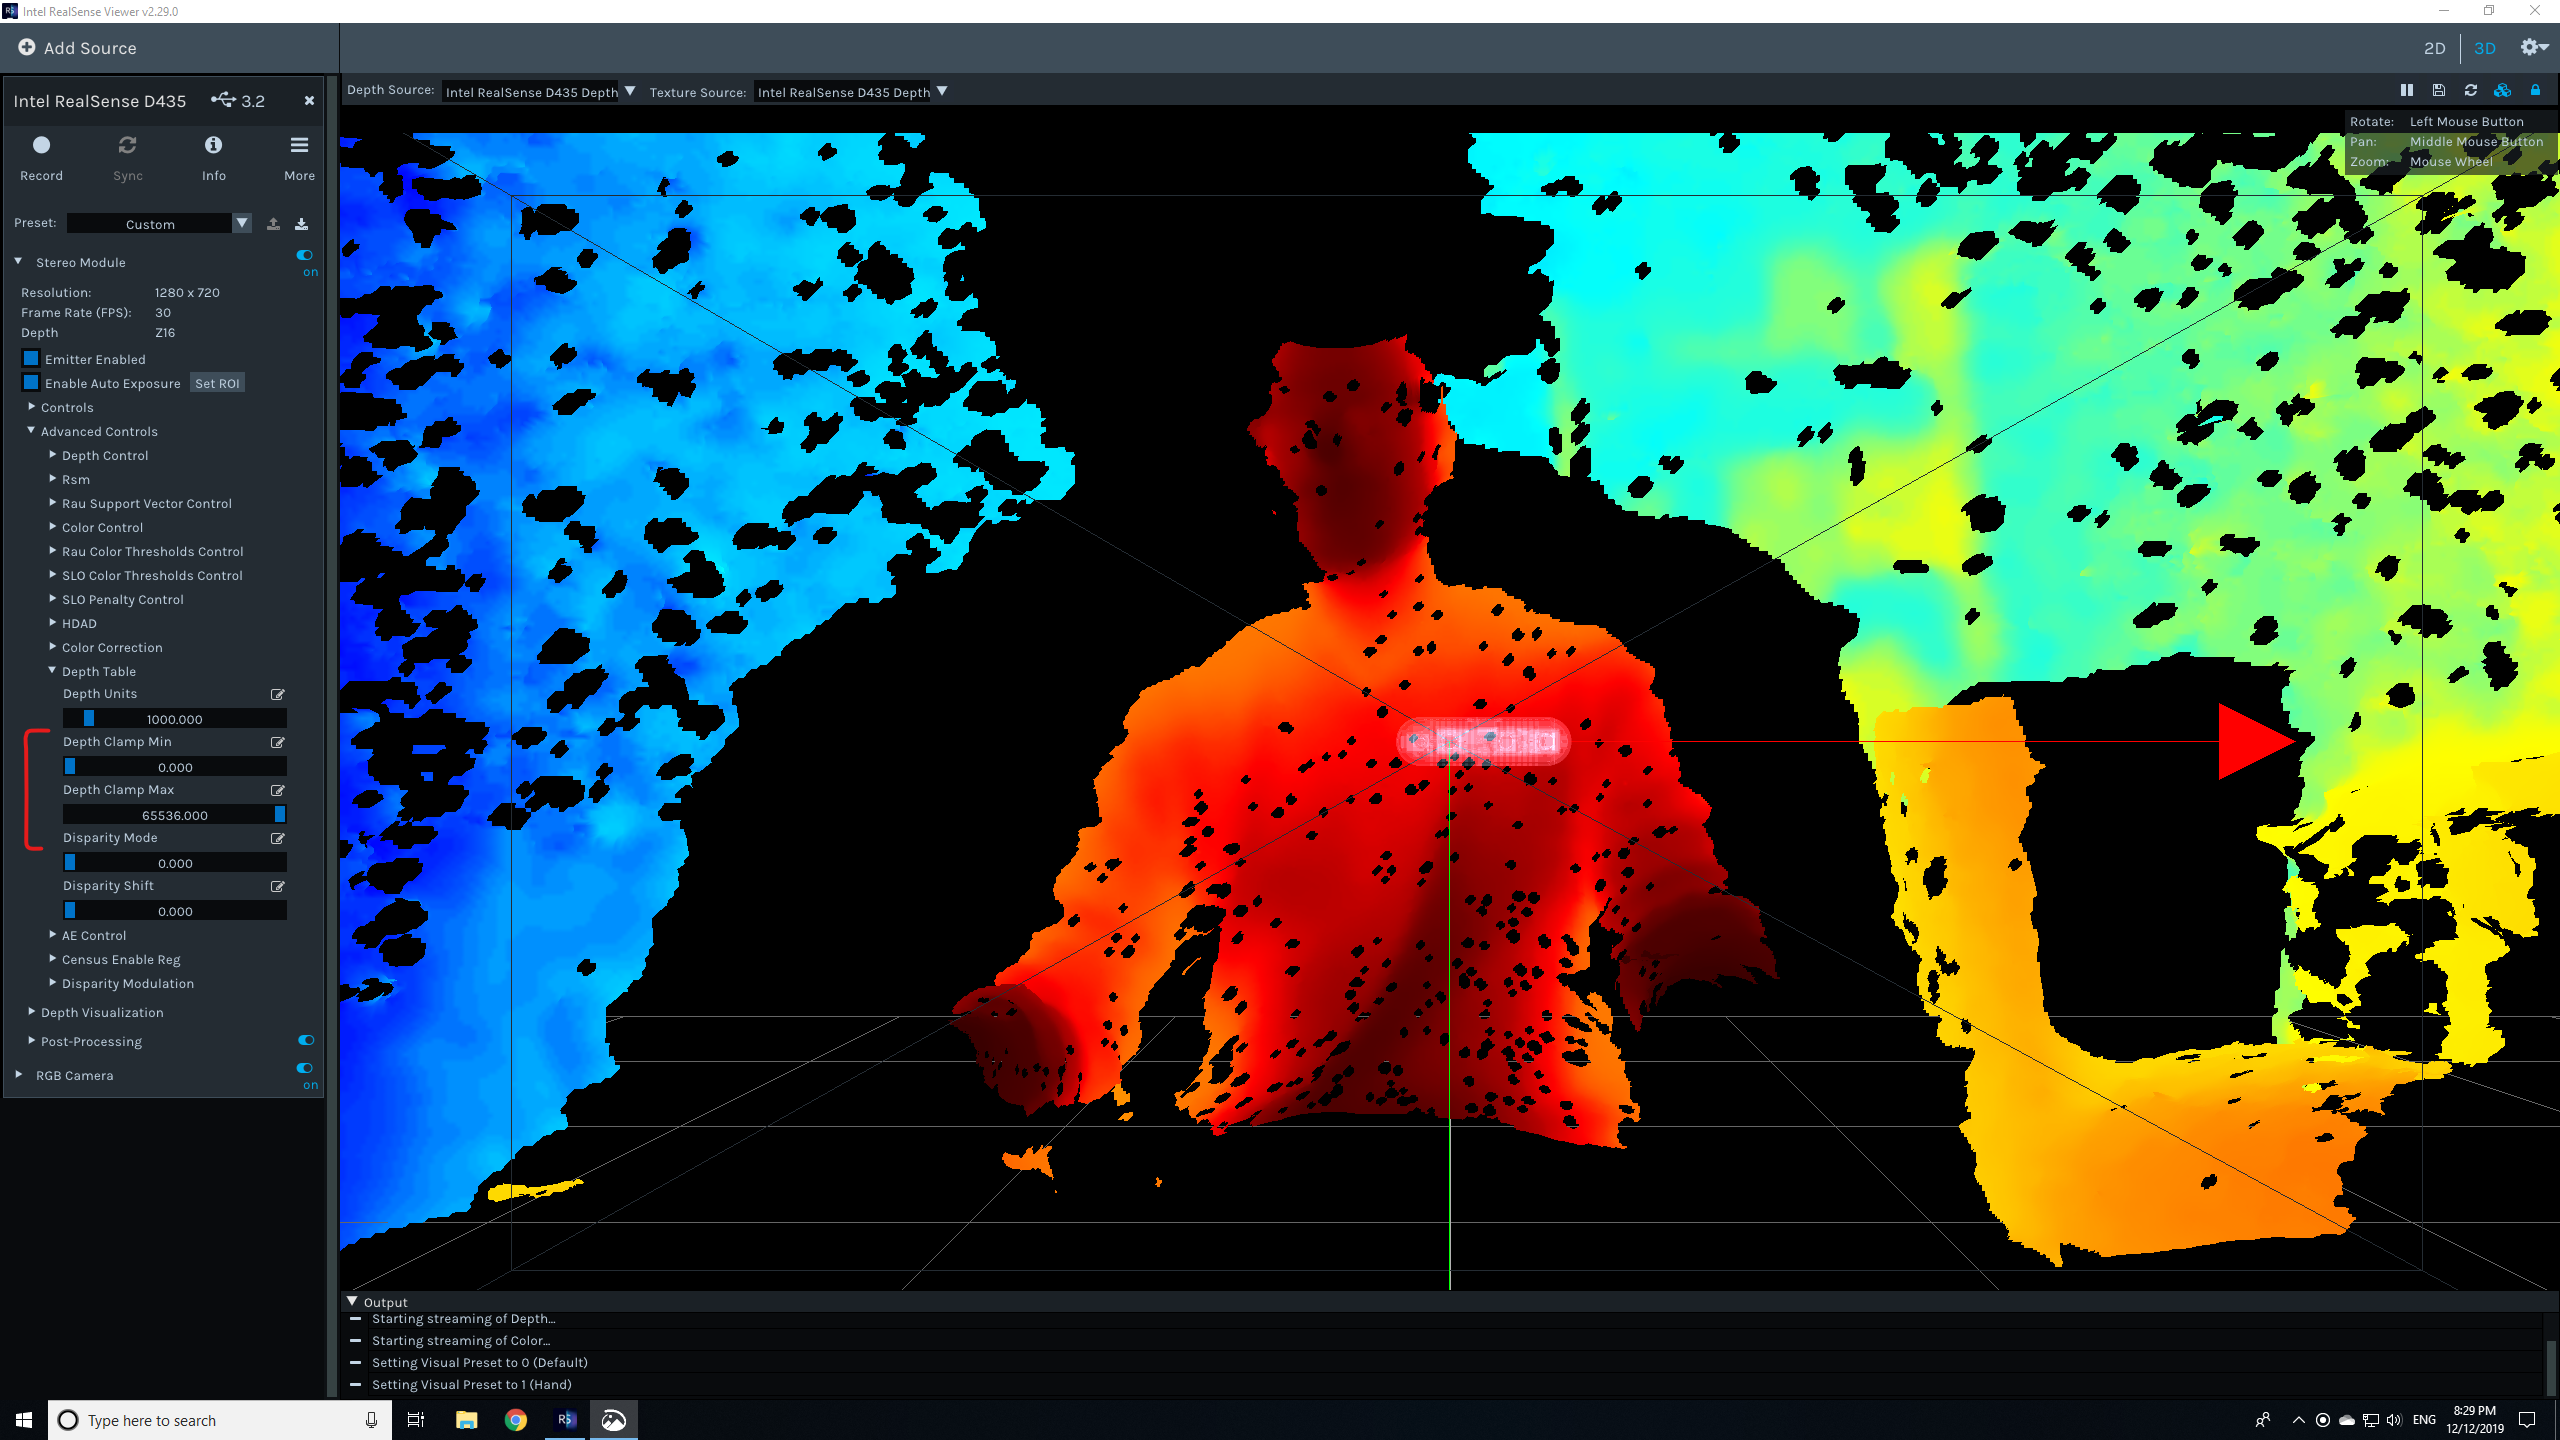
\includegraphics[width=0.45\textwidth]{max_depth_1.png}
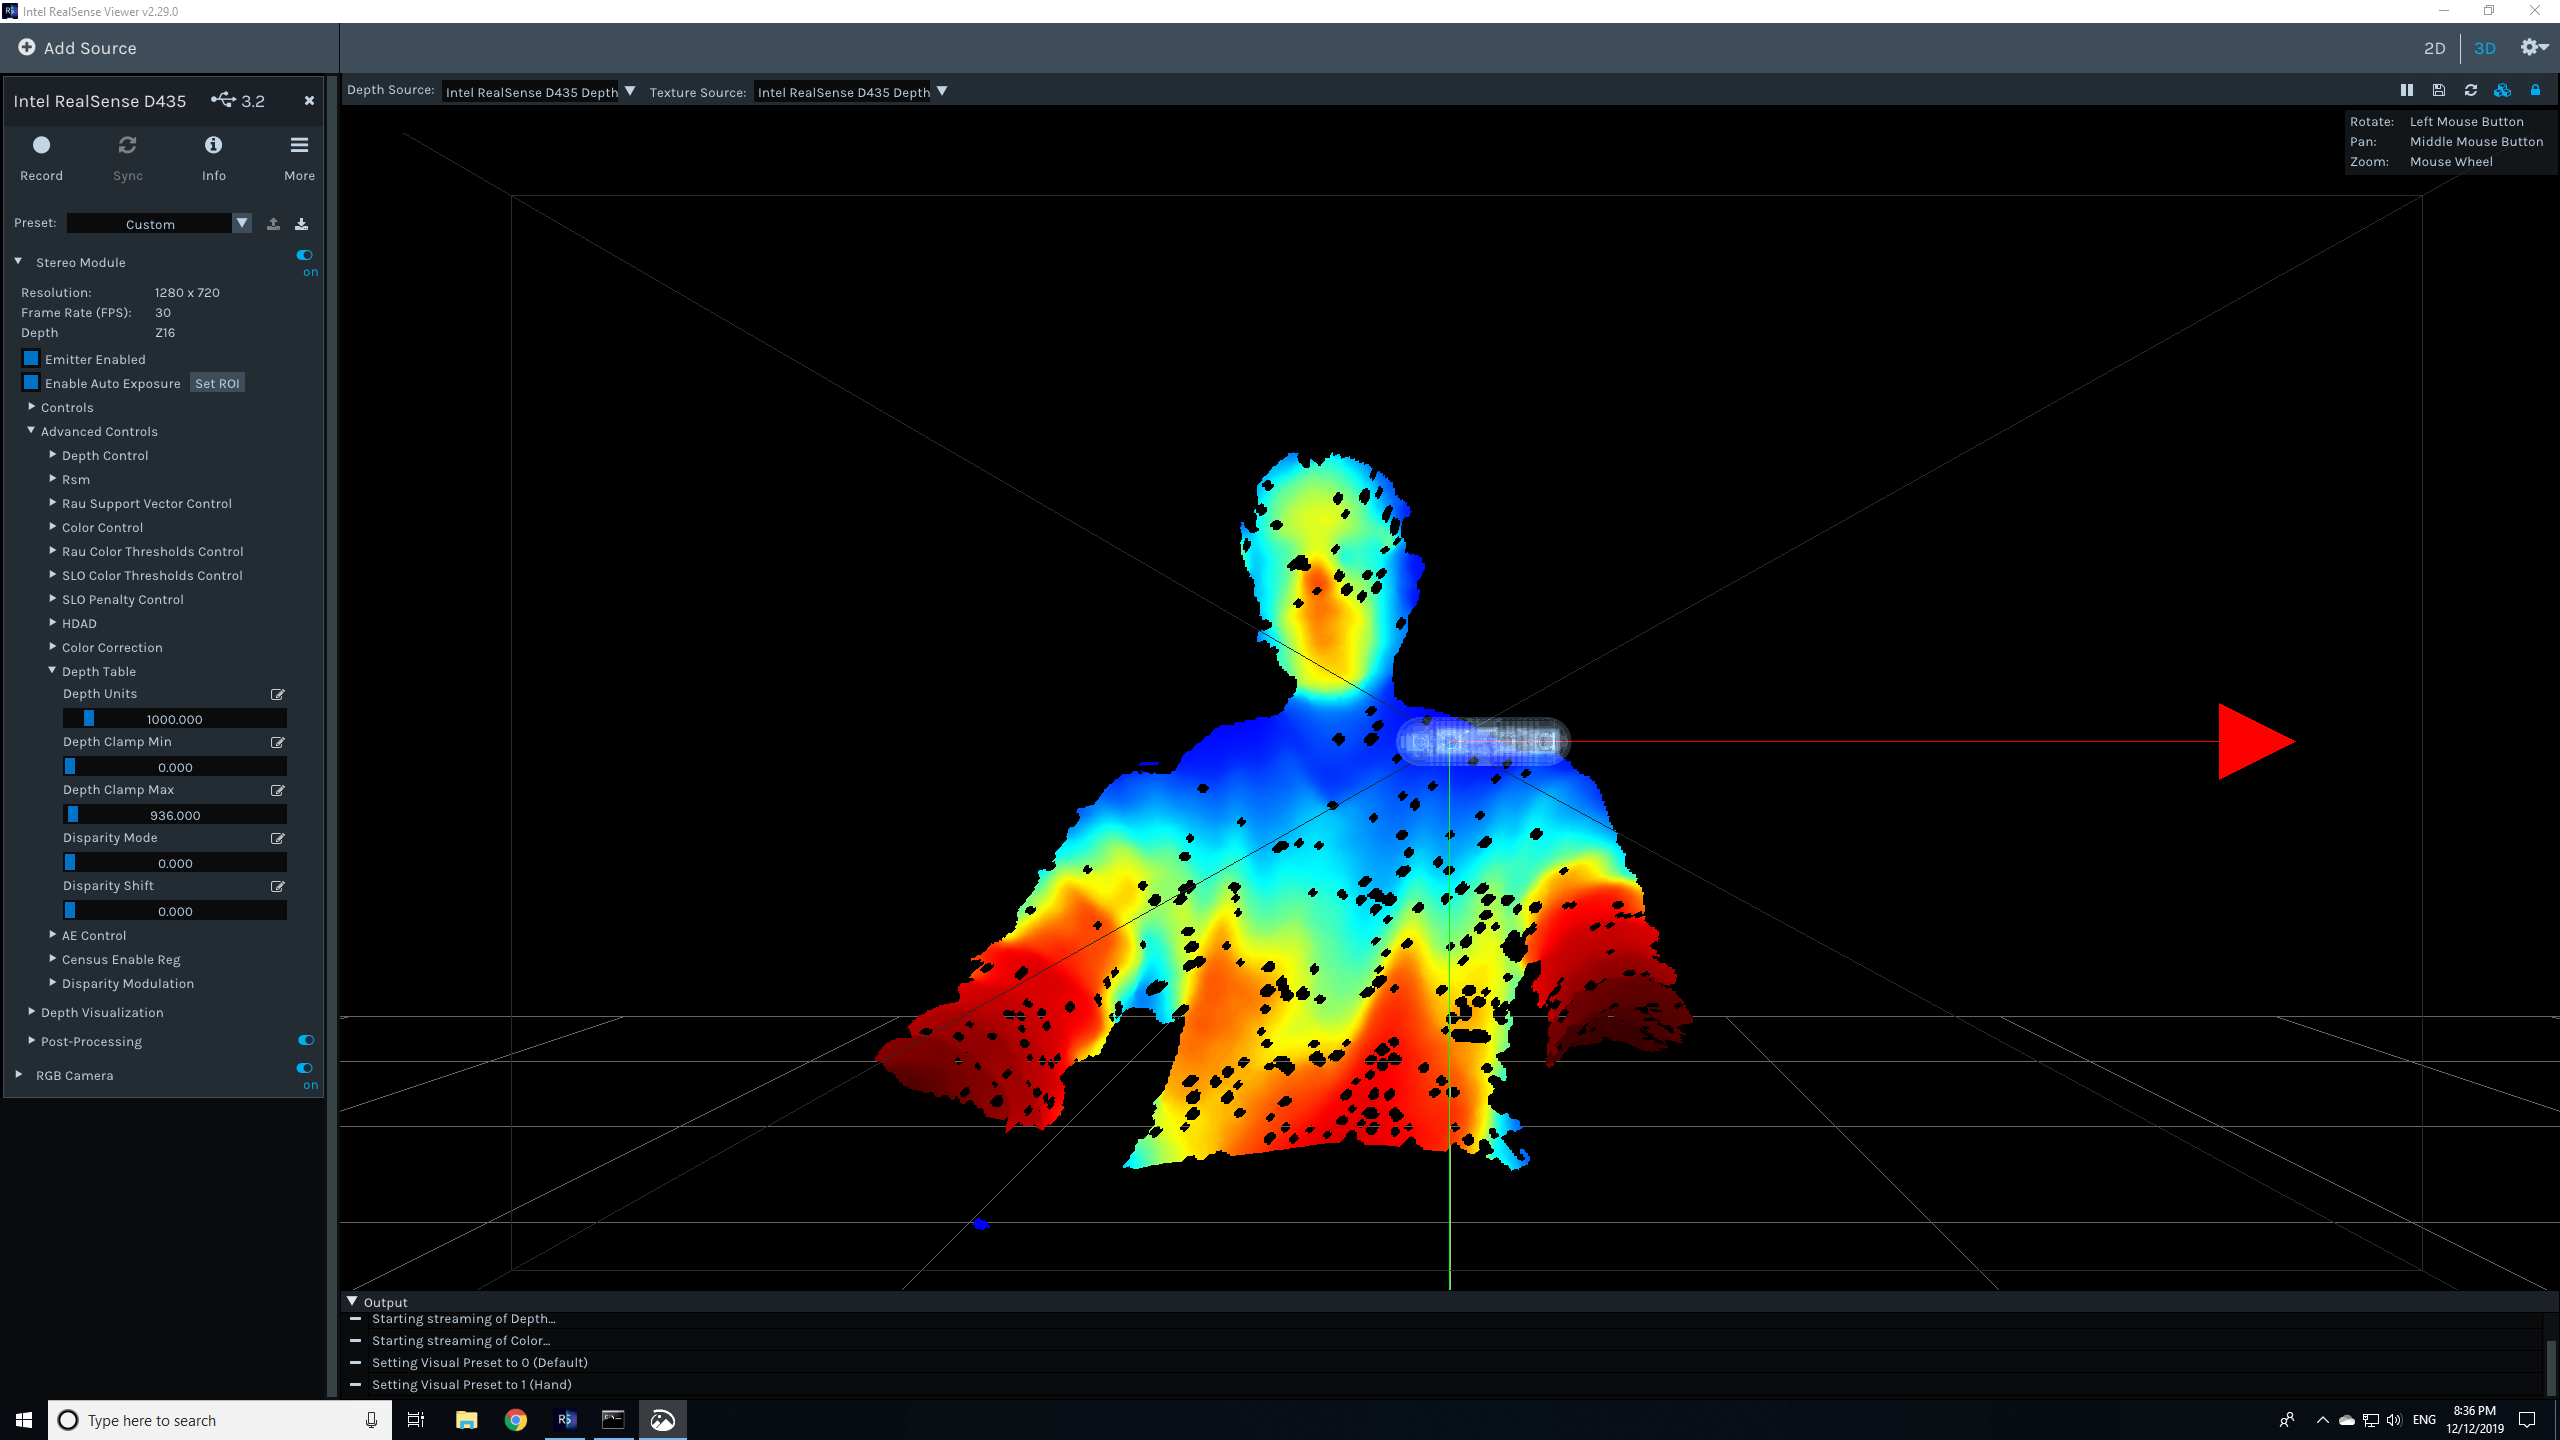
\includegraphics[width=0.45\textwidth]{max_depth_2.png}
\caption{Culling the back wall with max depth clamp}
\end{figure}

The RealSense Viewer allows the user
to pause a 3d scene and export a point cloud to ``.ply'' format. It's also possible to do this programmatically using the SDK: a modified version of the librealsense \text{pointcloud} example
takes a number of delayed snapshots (included in appendix \ref{appendix:snapshots}).

\subsection{Filters}

The SDK and Viewer offer several post-processing filters to improve the quality of
the captured depth data. The spatial filter compares each pixel to its neighbours in a
frame to ensure that there are no improbable measurements. Temporal filters
compare new frames to some average or distribution of previous ones. The temporal
filter in particular reduces the flickering and warping of depth streams.

\begin{figure}[h]
\centering
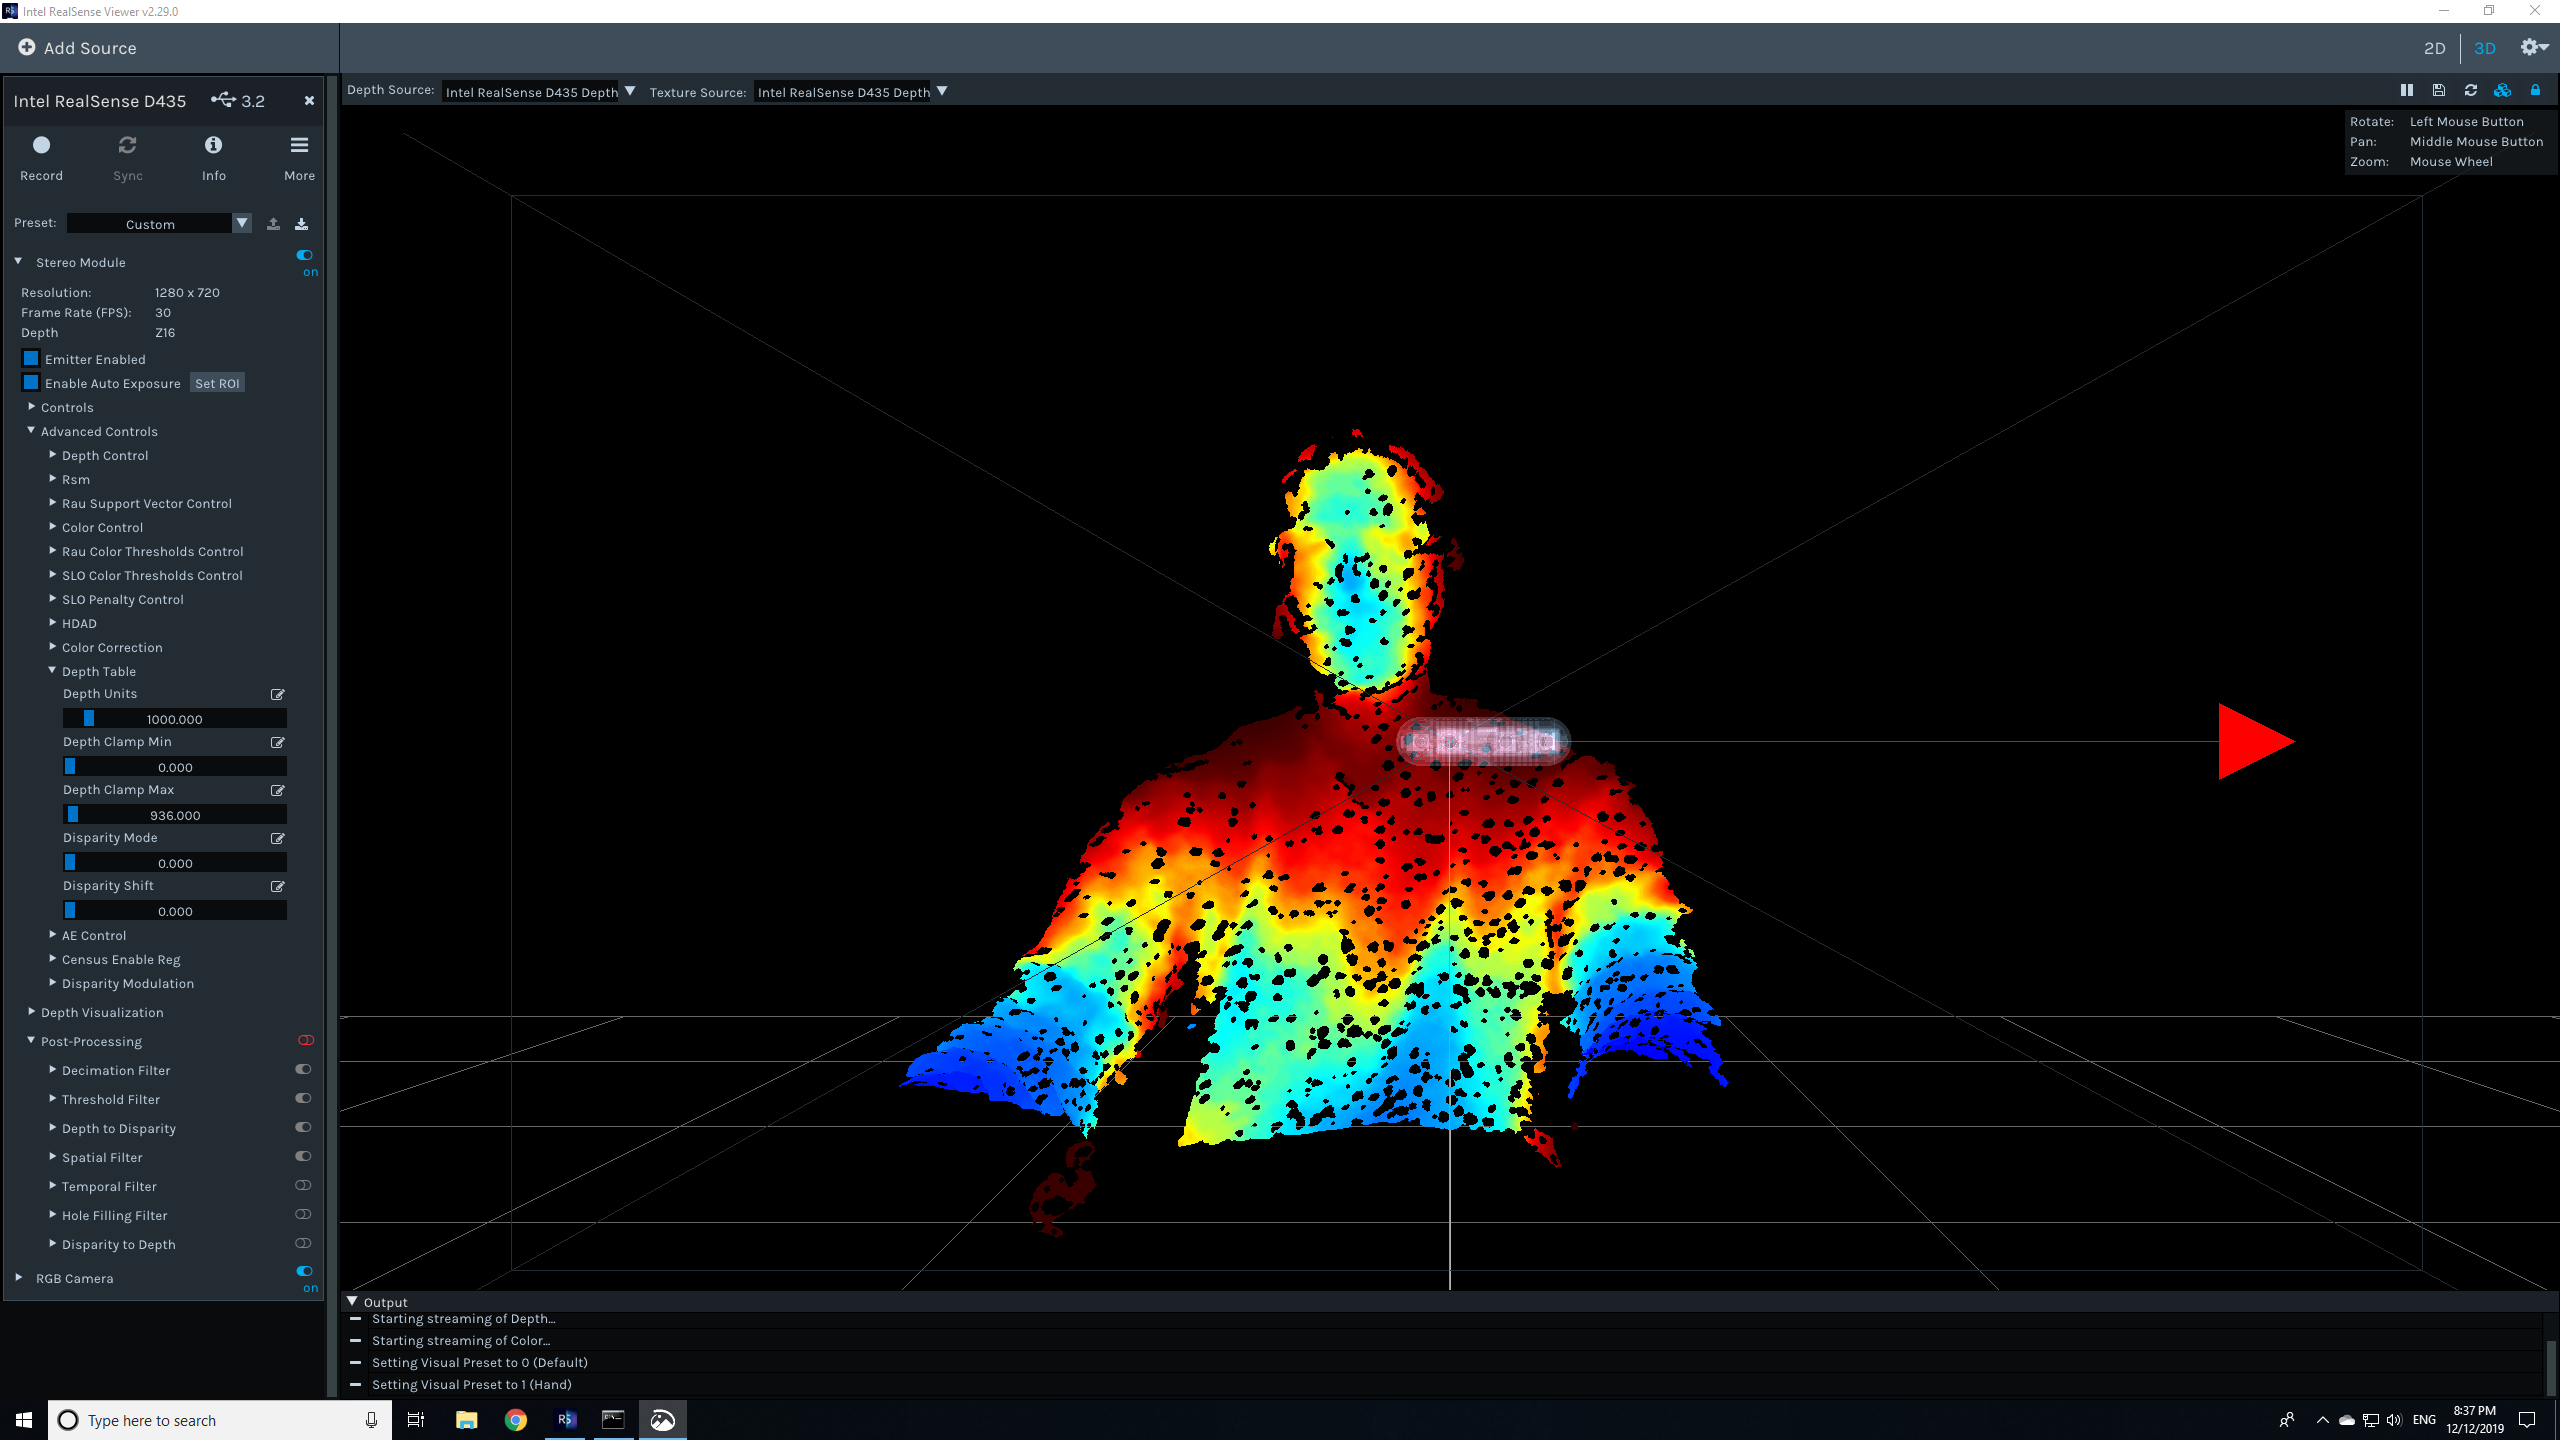
\includegraphics[width=0.3\textwidth]{without_post_processing.png}
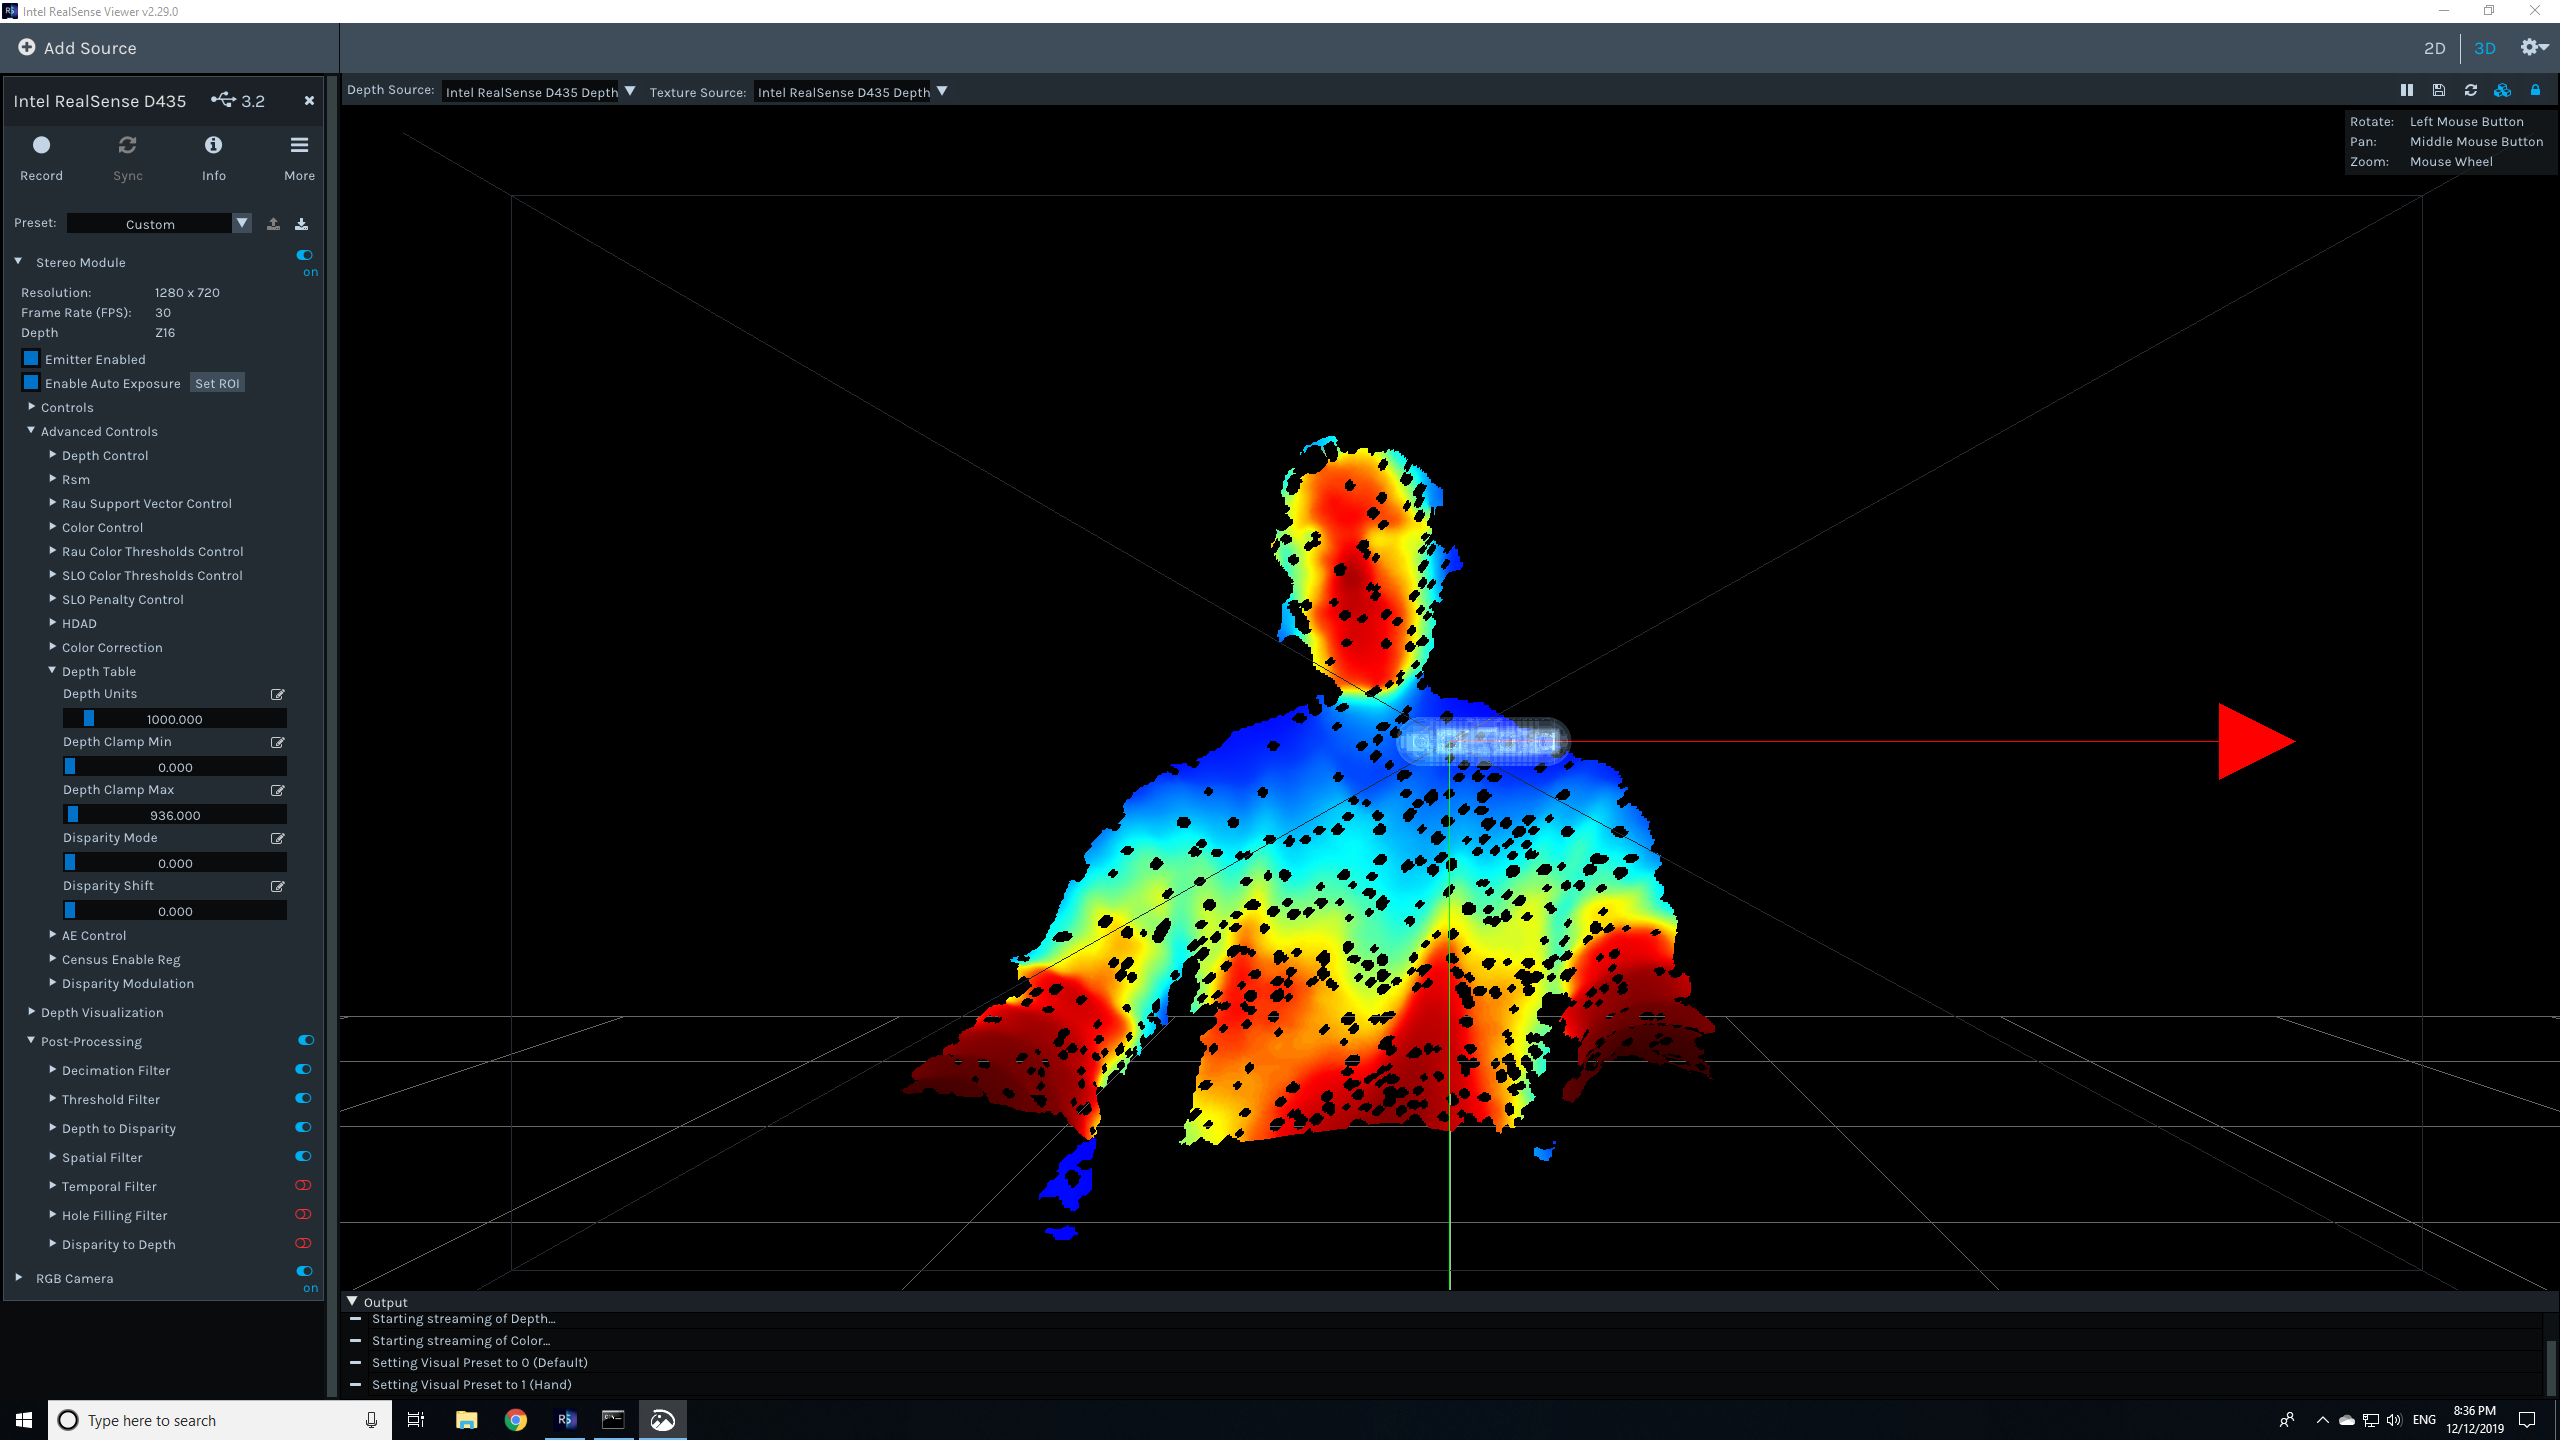
\includegraphics[width=0.3\textwidth]{with_spatial_filtering.png}
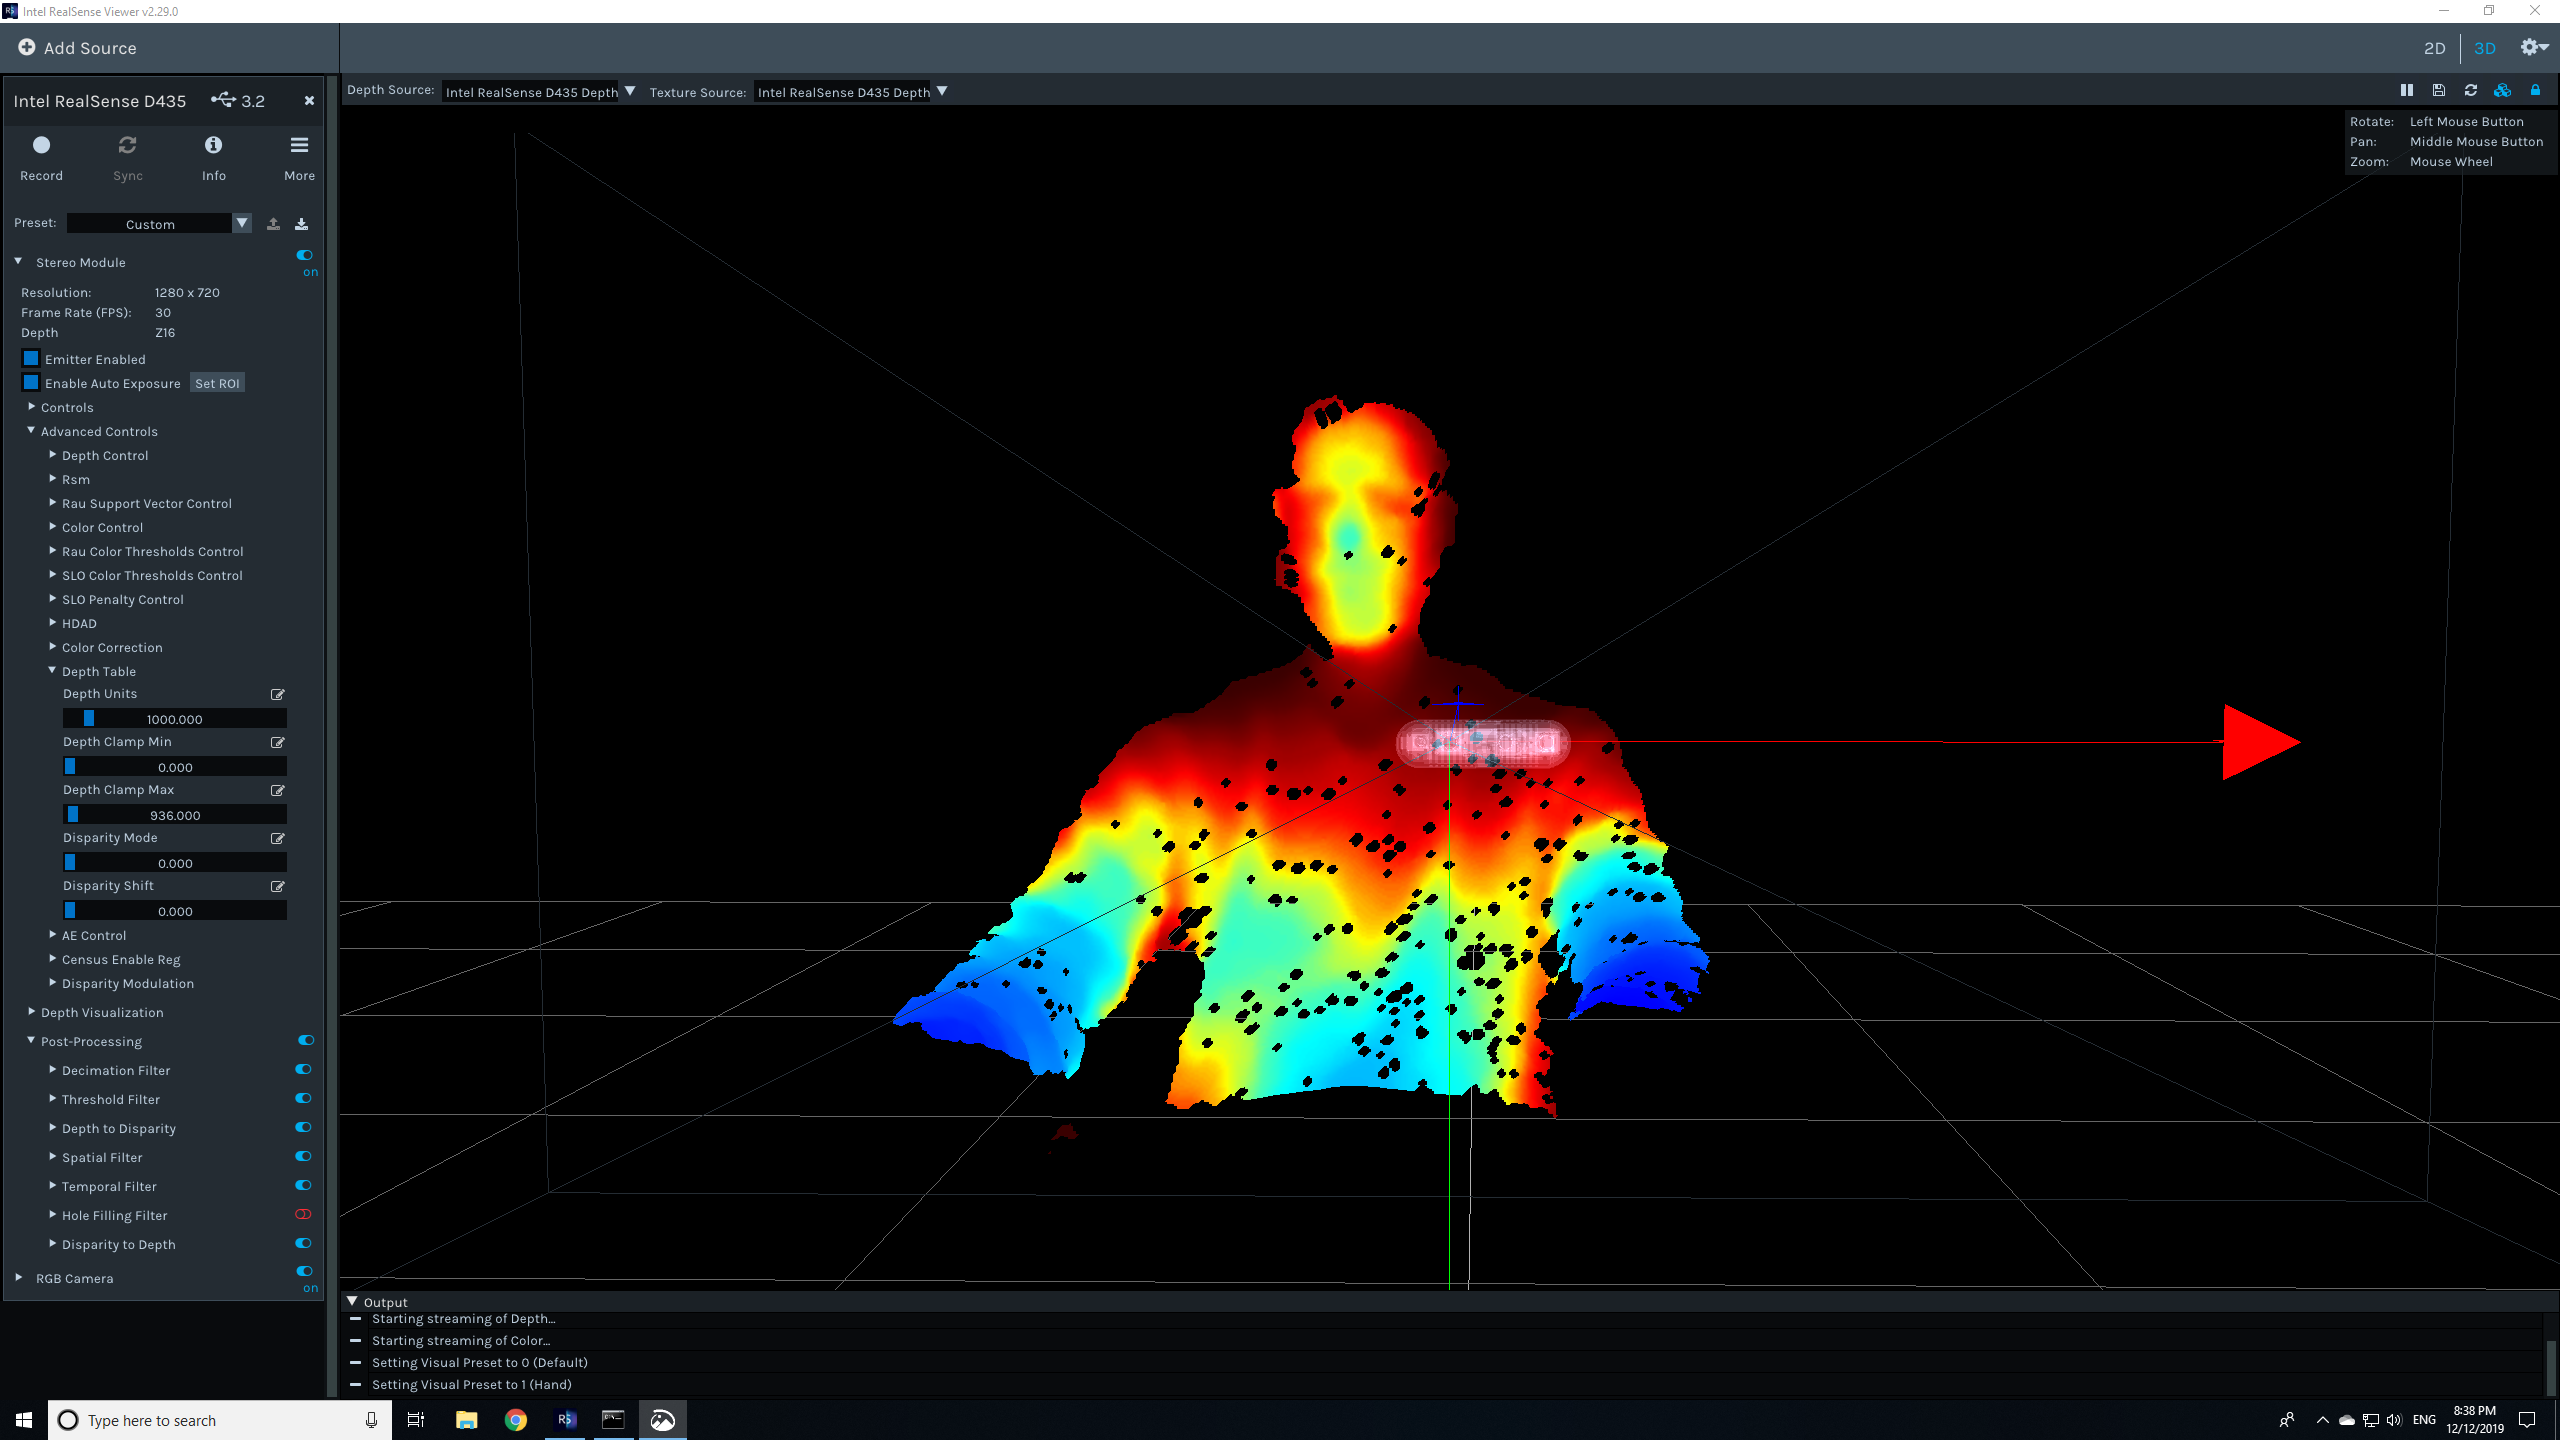
\includegraphics[width=0.3\textwidth]{with_all_processing_but_hole_filling.png}
\caption{Depth images captured without post processing (left), with spatial filtering (middle)
and using all available options (right)}
\end{figure}

Larger scale version of these images are included in Appendix \ref{appendix:postprocessing}.

\subsection{Removing Outliers and Errors}

Even with the background subtraction and filters, there are often still
outliers and errors that should not be included in a quality model. Worse still,
these garbage vertices make it harder to perform the registration in the next phase.
Luckily, MeshLab \cite{cignoni2008meshlab} makes it quite easy to select,
move and delete vertices.

\begin{figure}[h]
\centering
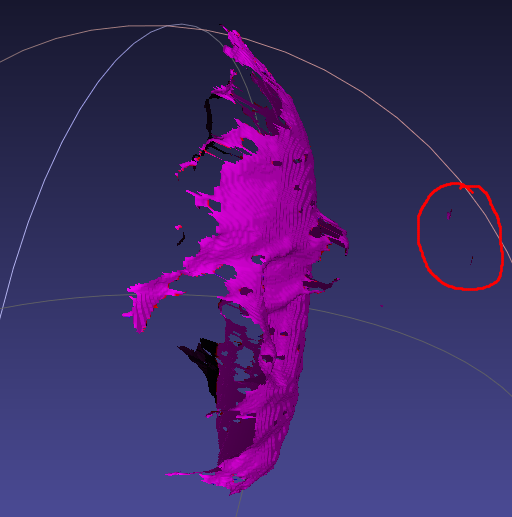
\includegraphics[width=0.45\textwidth]{outliers.png}
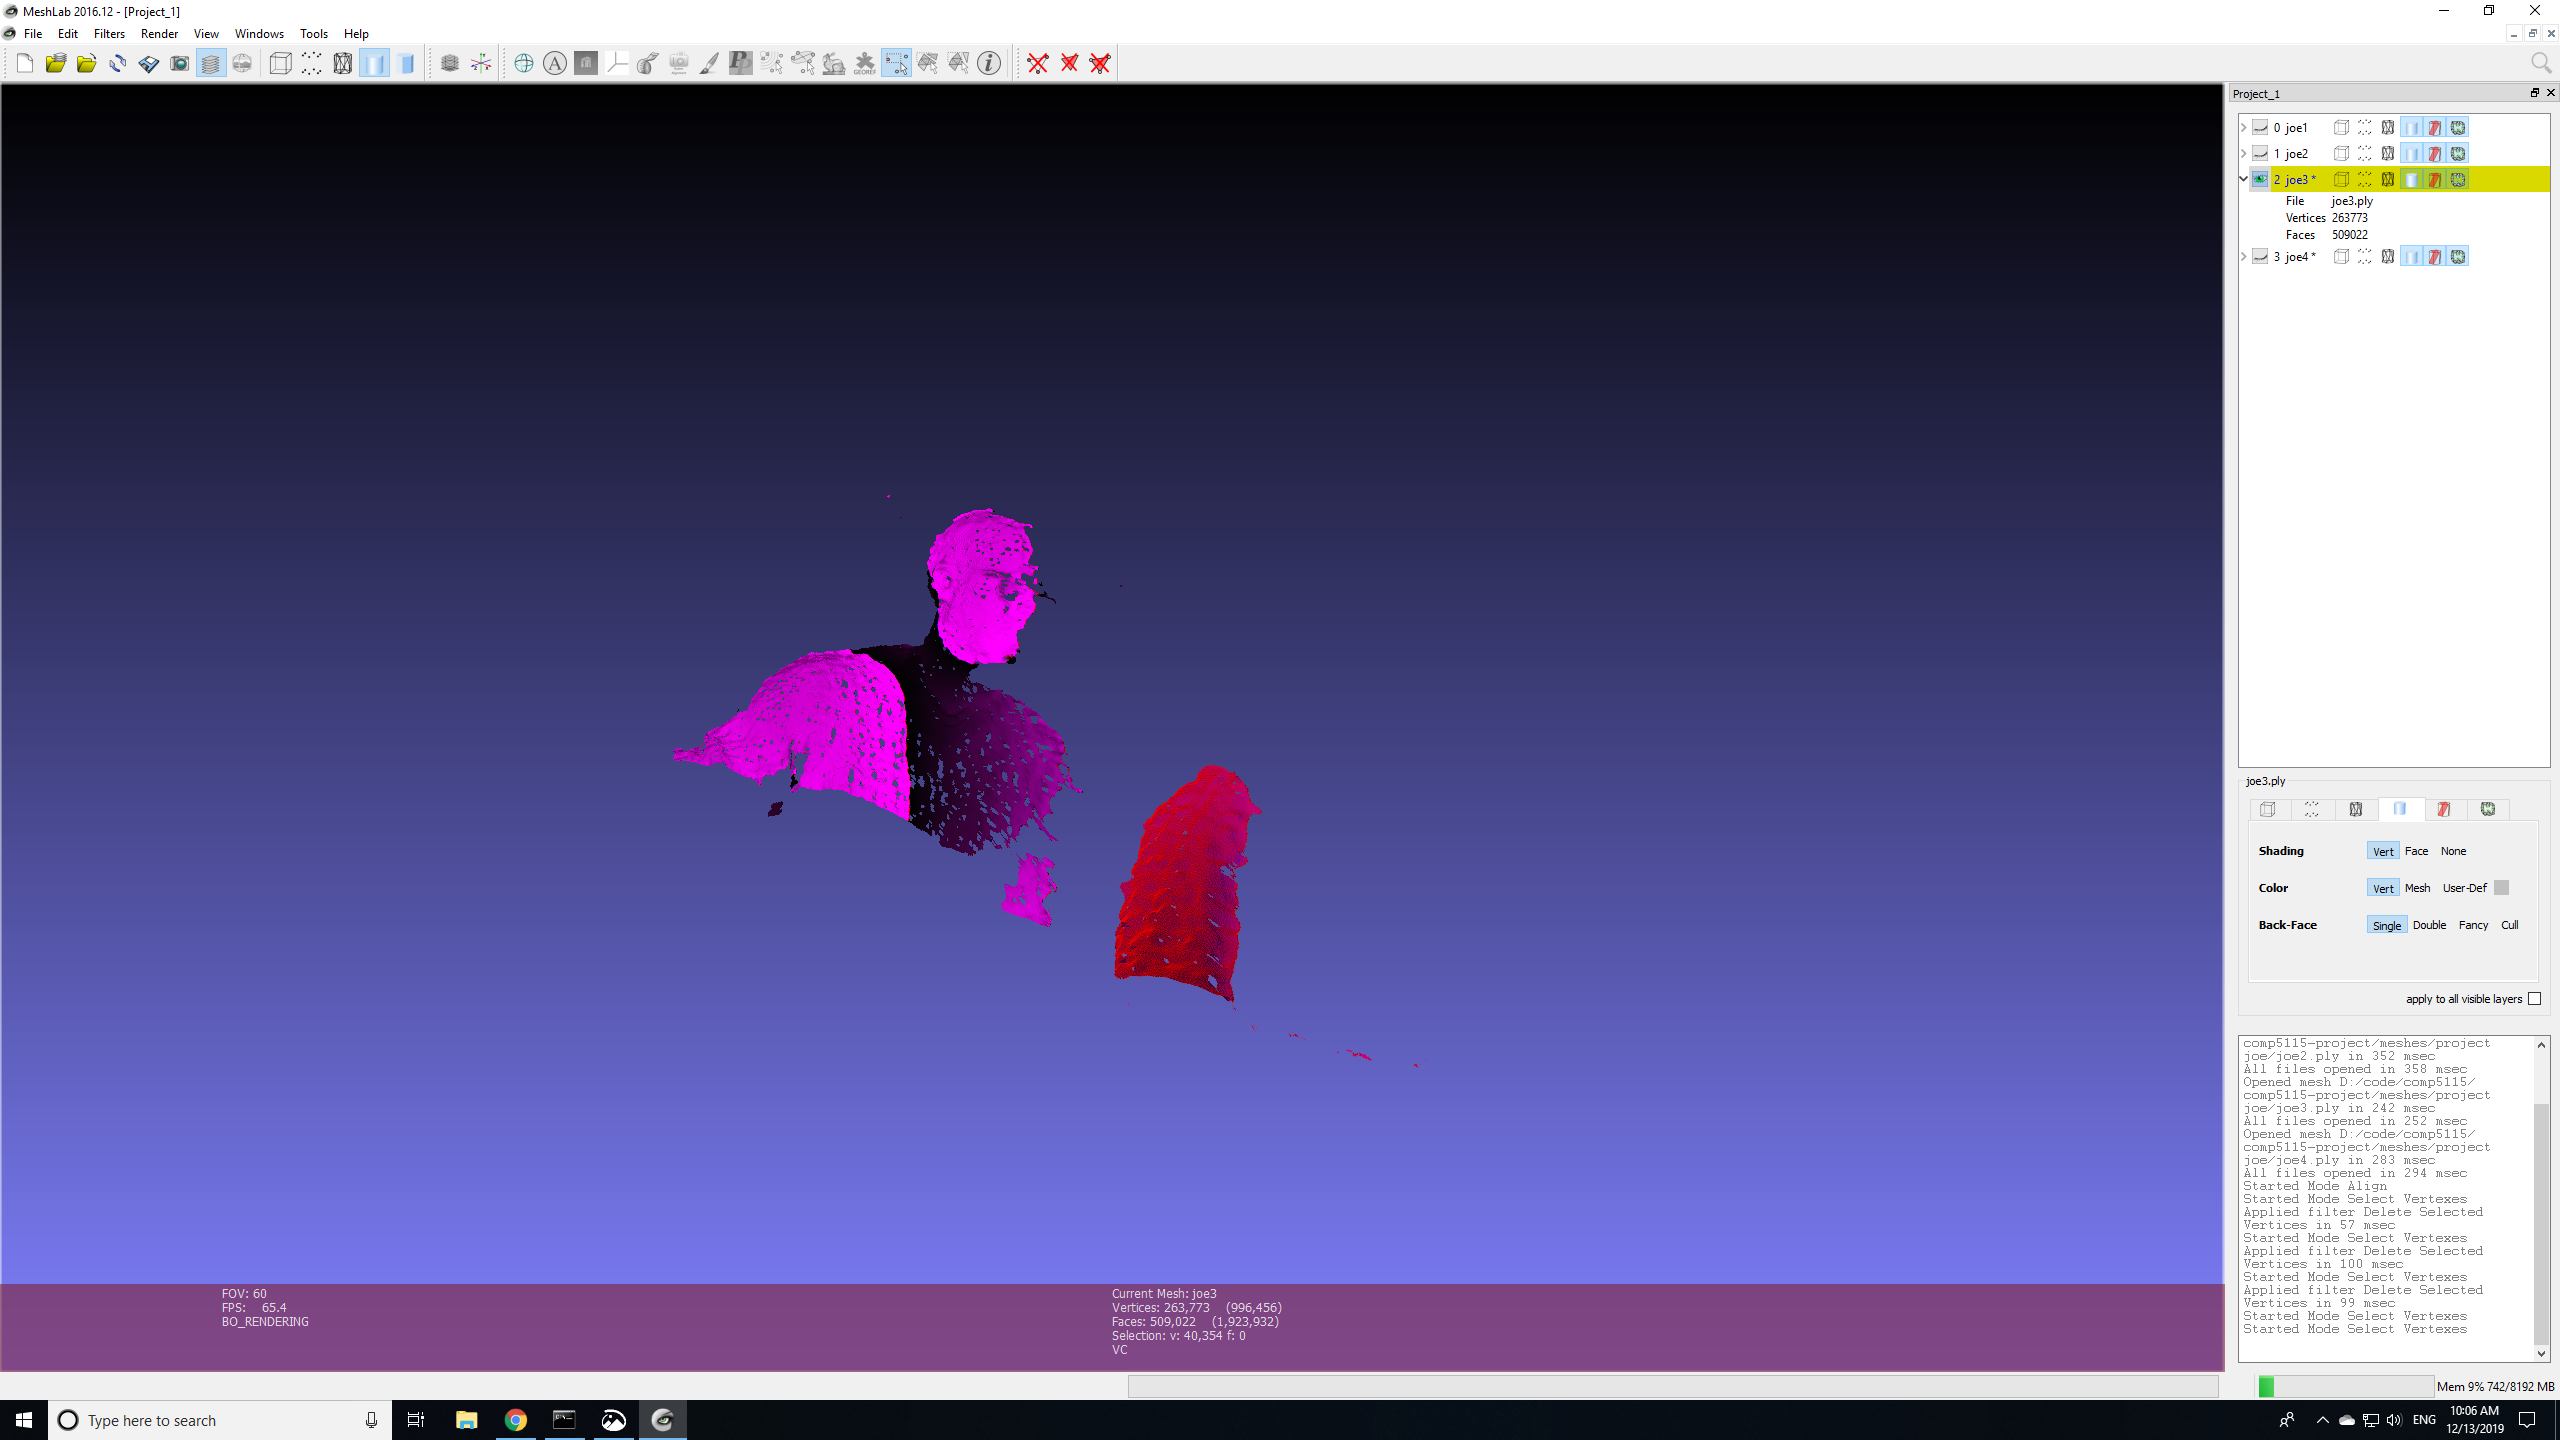
\includegraphics[width=0.45\textwidth]{removing_chair_from_layer.png}
\caption{Outliers caused by erroneous readings (left), removing chair from capture}
\end{figure}

One way to remove extraneous points is to use the connected component selection
tool to grab the object of interest, then use the selection inversion to select
every point except the model. All these vertices and/or faces can then be deleted.

This process needs to be repeated for each point cloud which will constitute
a ``layer'' in the model construction.

\subsection{Aligning Point Clouds}

Once cleaned, MeshLab \cite{cignoni2008meshlab} can be used to align the point clouds.
Each point cloud mesh is imported as its own layed, which can be moved and rotated so that
they lign up closely. This problem is also known as point cloud registration \cite{pomerleau2015review} and the Iterative
Closest Points (or ICP) is another well-studied algorithm. MeshLab provides a user-assisted
method for giving the ICP a head start by choosing an initial alignment.

In MeshLab, open the Alignment tool and Glue one of the layers as a base.
Now choose a different layer to align and select Point Based Gluing.
It opens a new window which allows the user to move and rotate the two clouds to better view
common areas. Then, the user selects (at least) four points corresponding points on
both of the models to find an initial alignment.
Often, this initial alignment is not correct and the user must try again
with different points.

\begin{figure}[h]
\centering
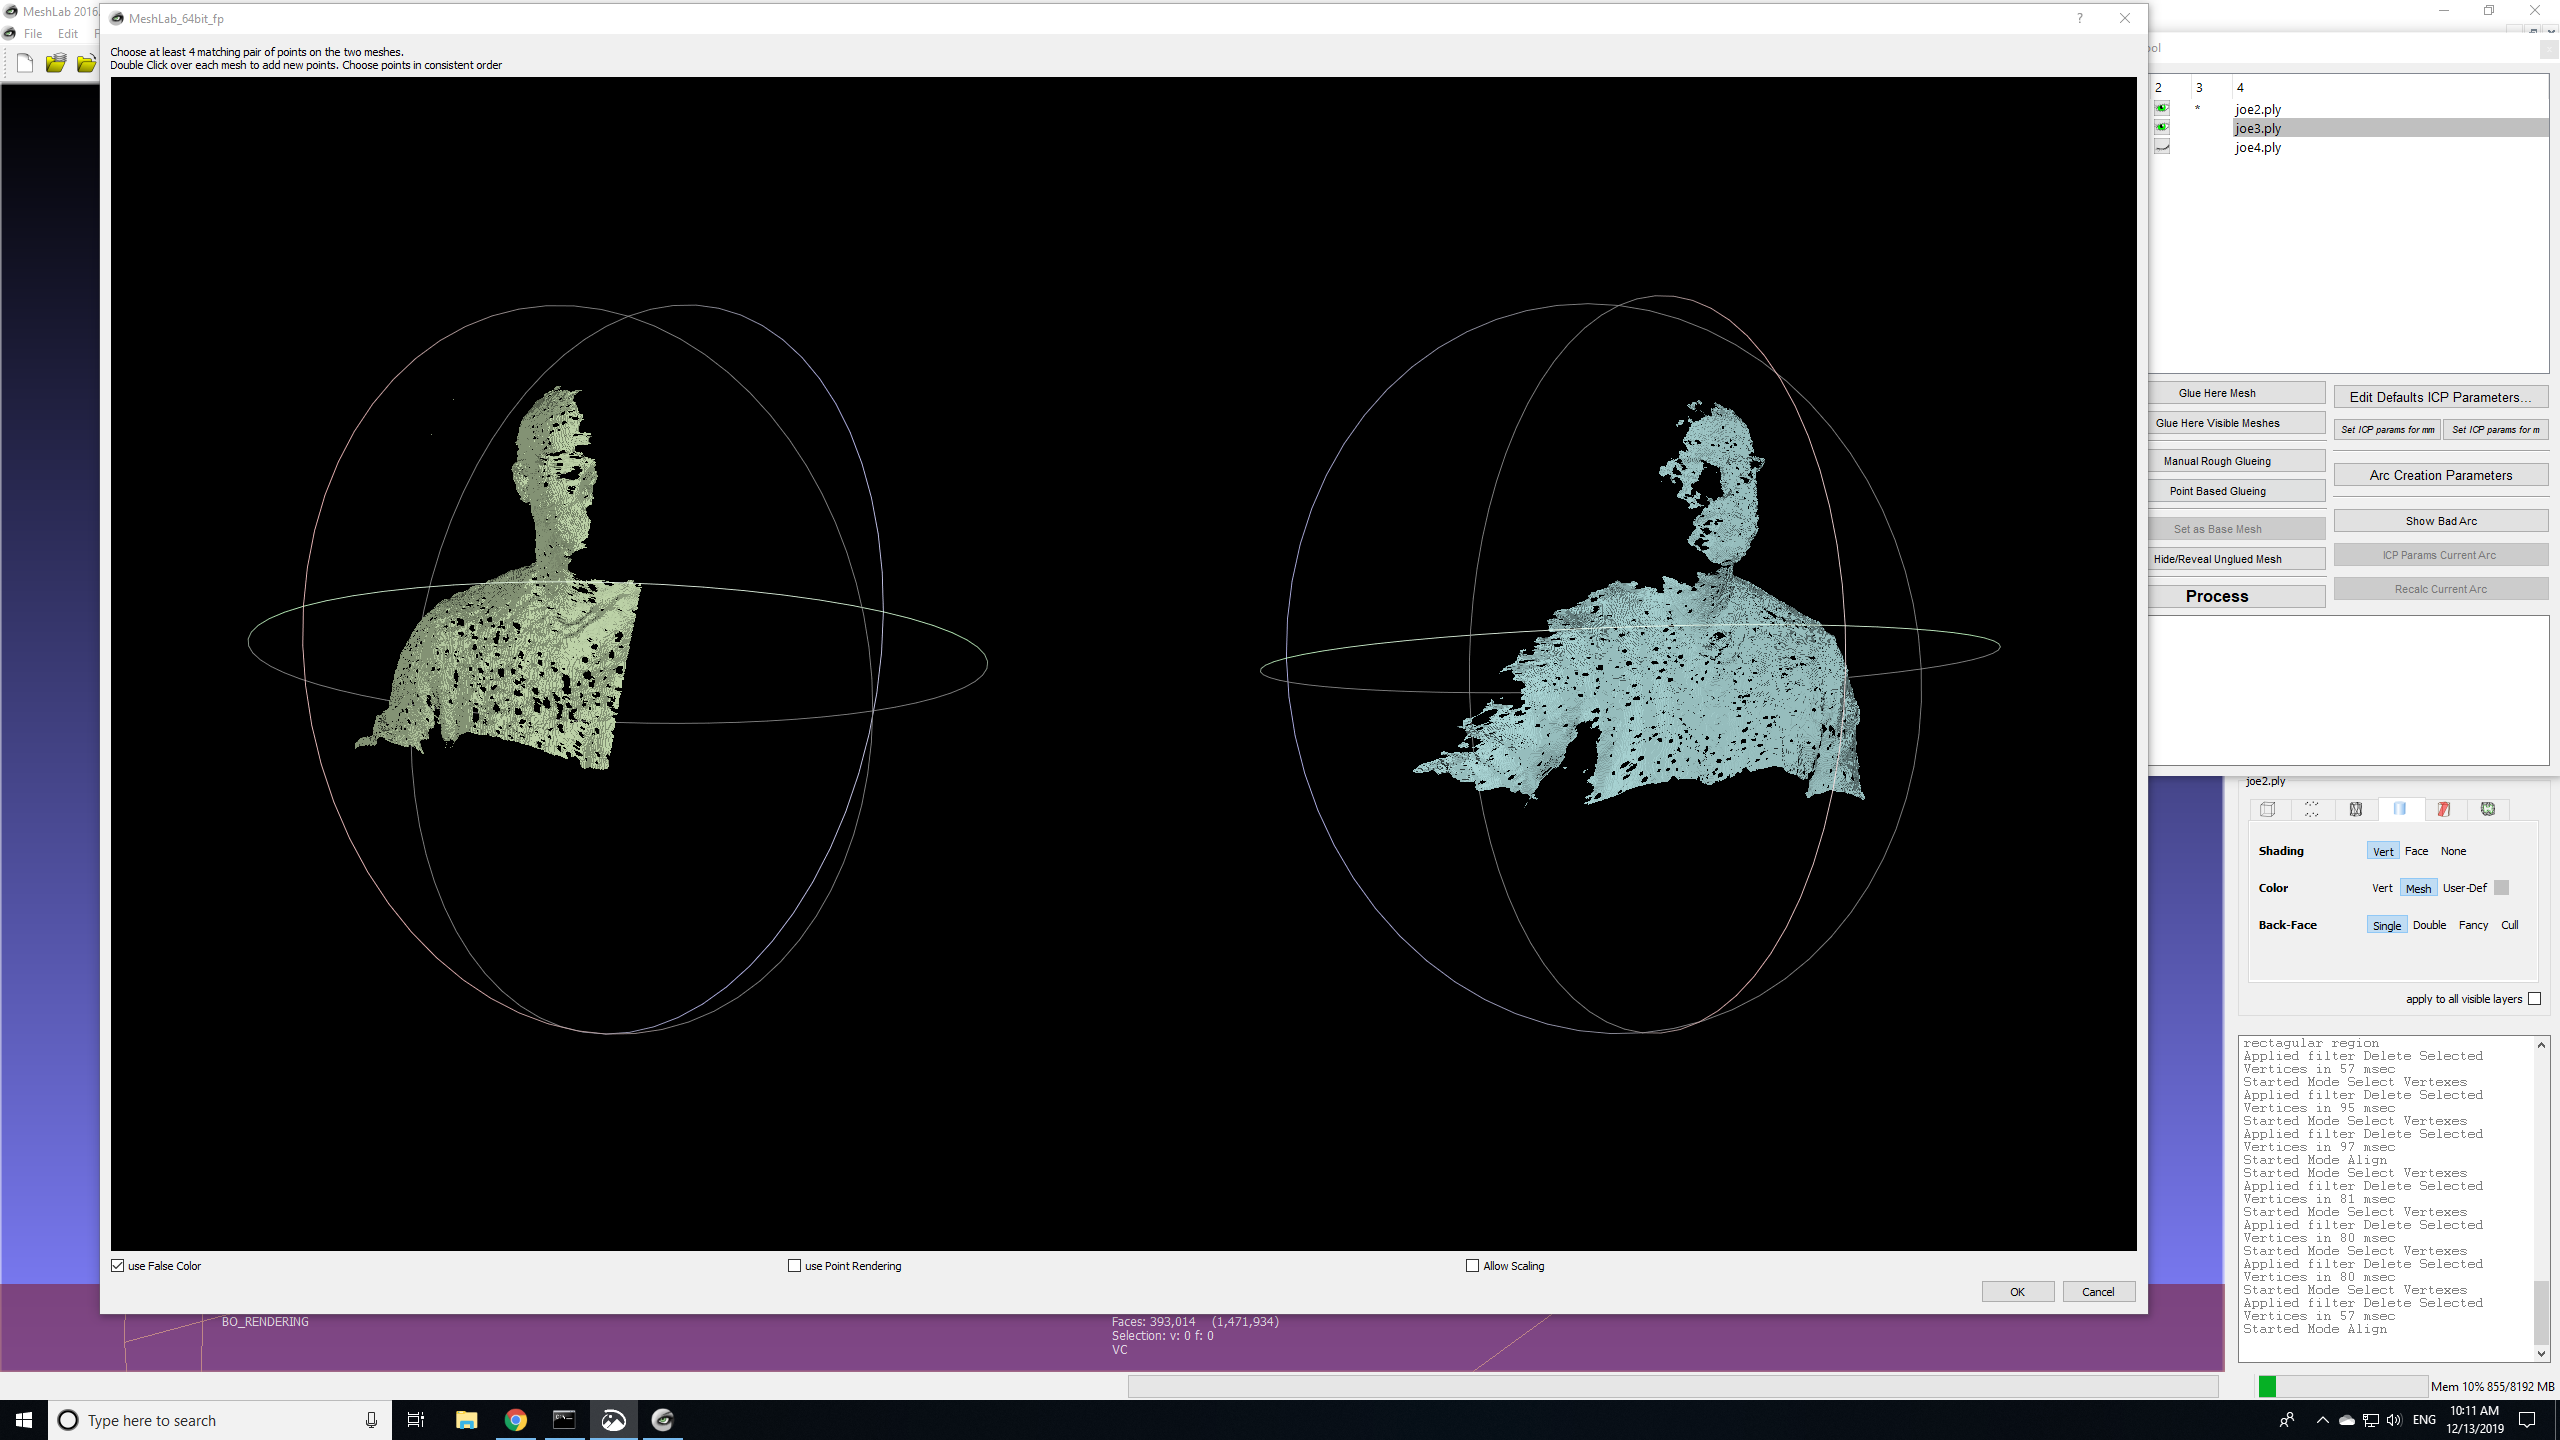
\includegraphics[width=0.6\textwidth]{align_two_clouds.png}
\caption{Point-based Initial Transform}
\end{figure}

Once an initial alignment is found, presssing Process in the Alignment window
runs Iterative Closest Points to refine the alignment. It is often helpful
to run the algorithm several times and/or increase the number of iterations in the
ICP parameters.

It can be particularly tricky to align two models with little in common. For a
quality point cloud, it would be necessary to take dozens if not hundreds
of captures so that the transition from each frame is smooth and common surface
between each one is maximized, especially if there are sharp edges as in the
Cube Man project.

\begin{figure}[H]
\centering
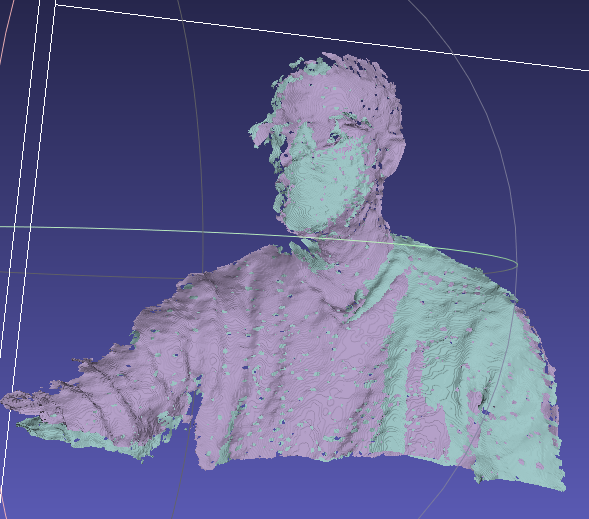
\includegraphics[width=0.6\textwidth]{two_clouds_merged.png}
\caption{Two point clouds aligned using ICP}
\end{figure}

After aligning two (or more) layers, you can then flatten them together by making
the aligned layers visible, right clicking in the layers window, and selecting
Flatten Visible Layers. Flattening the layers arguably makes it easier align additional
point clouds, since the known surface has hopefully expanded.

\subsection{Simplifications, Sampling and Smoothing}
Attempting reconstruction directly on the merged point clouds leads to fairly messy
objects. There are often non-manifold vertices and incorrect normals which will lead to
strange objects.

\begin{figure}[H]
\centering
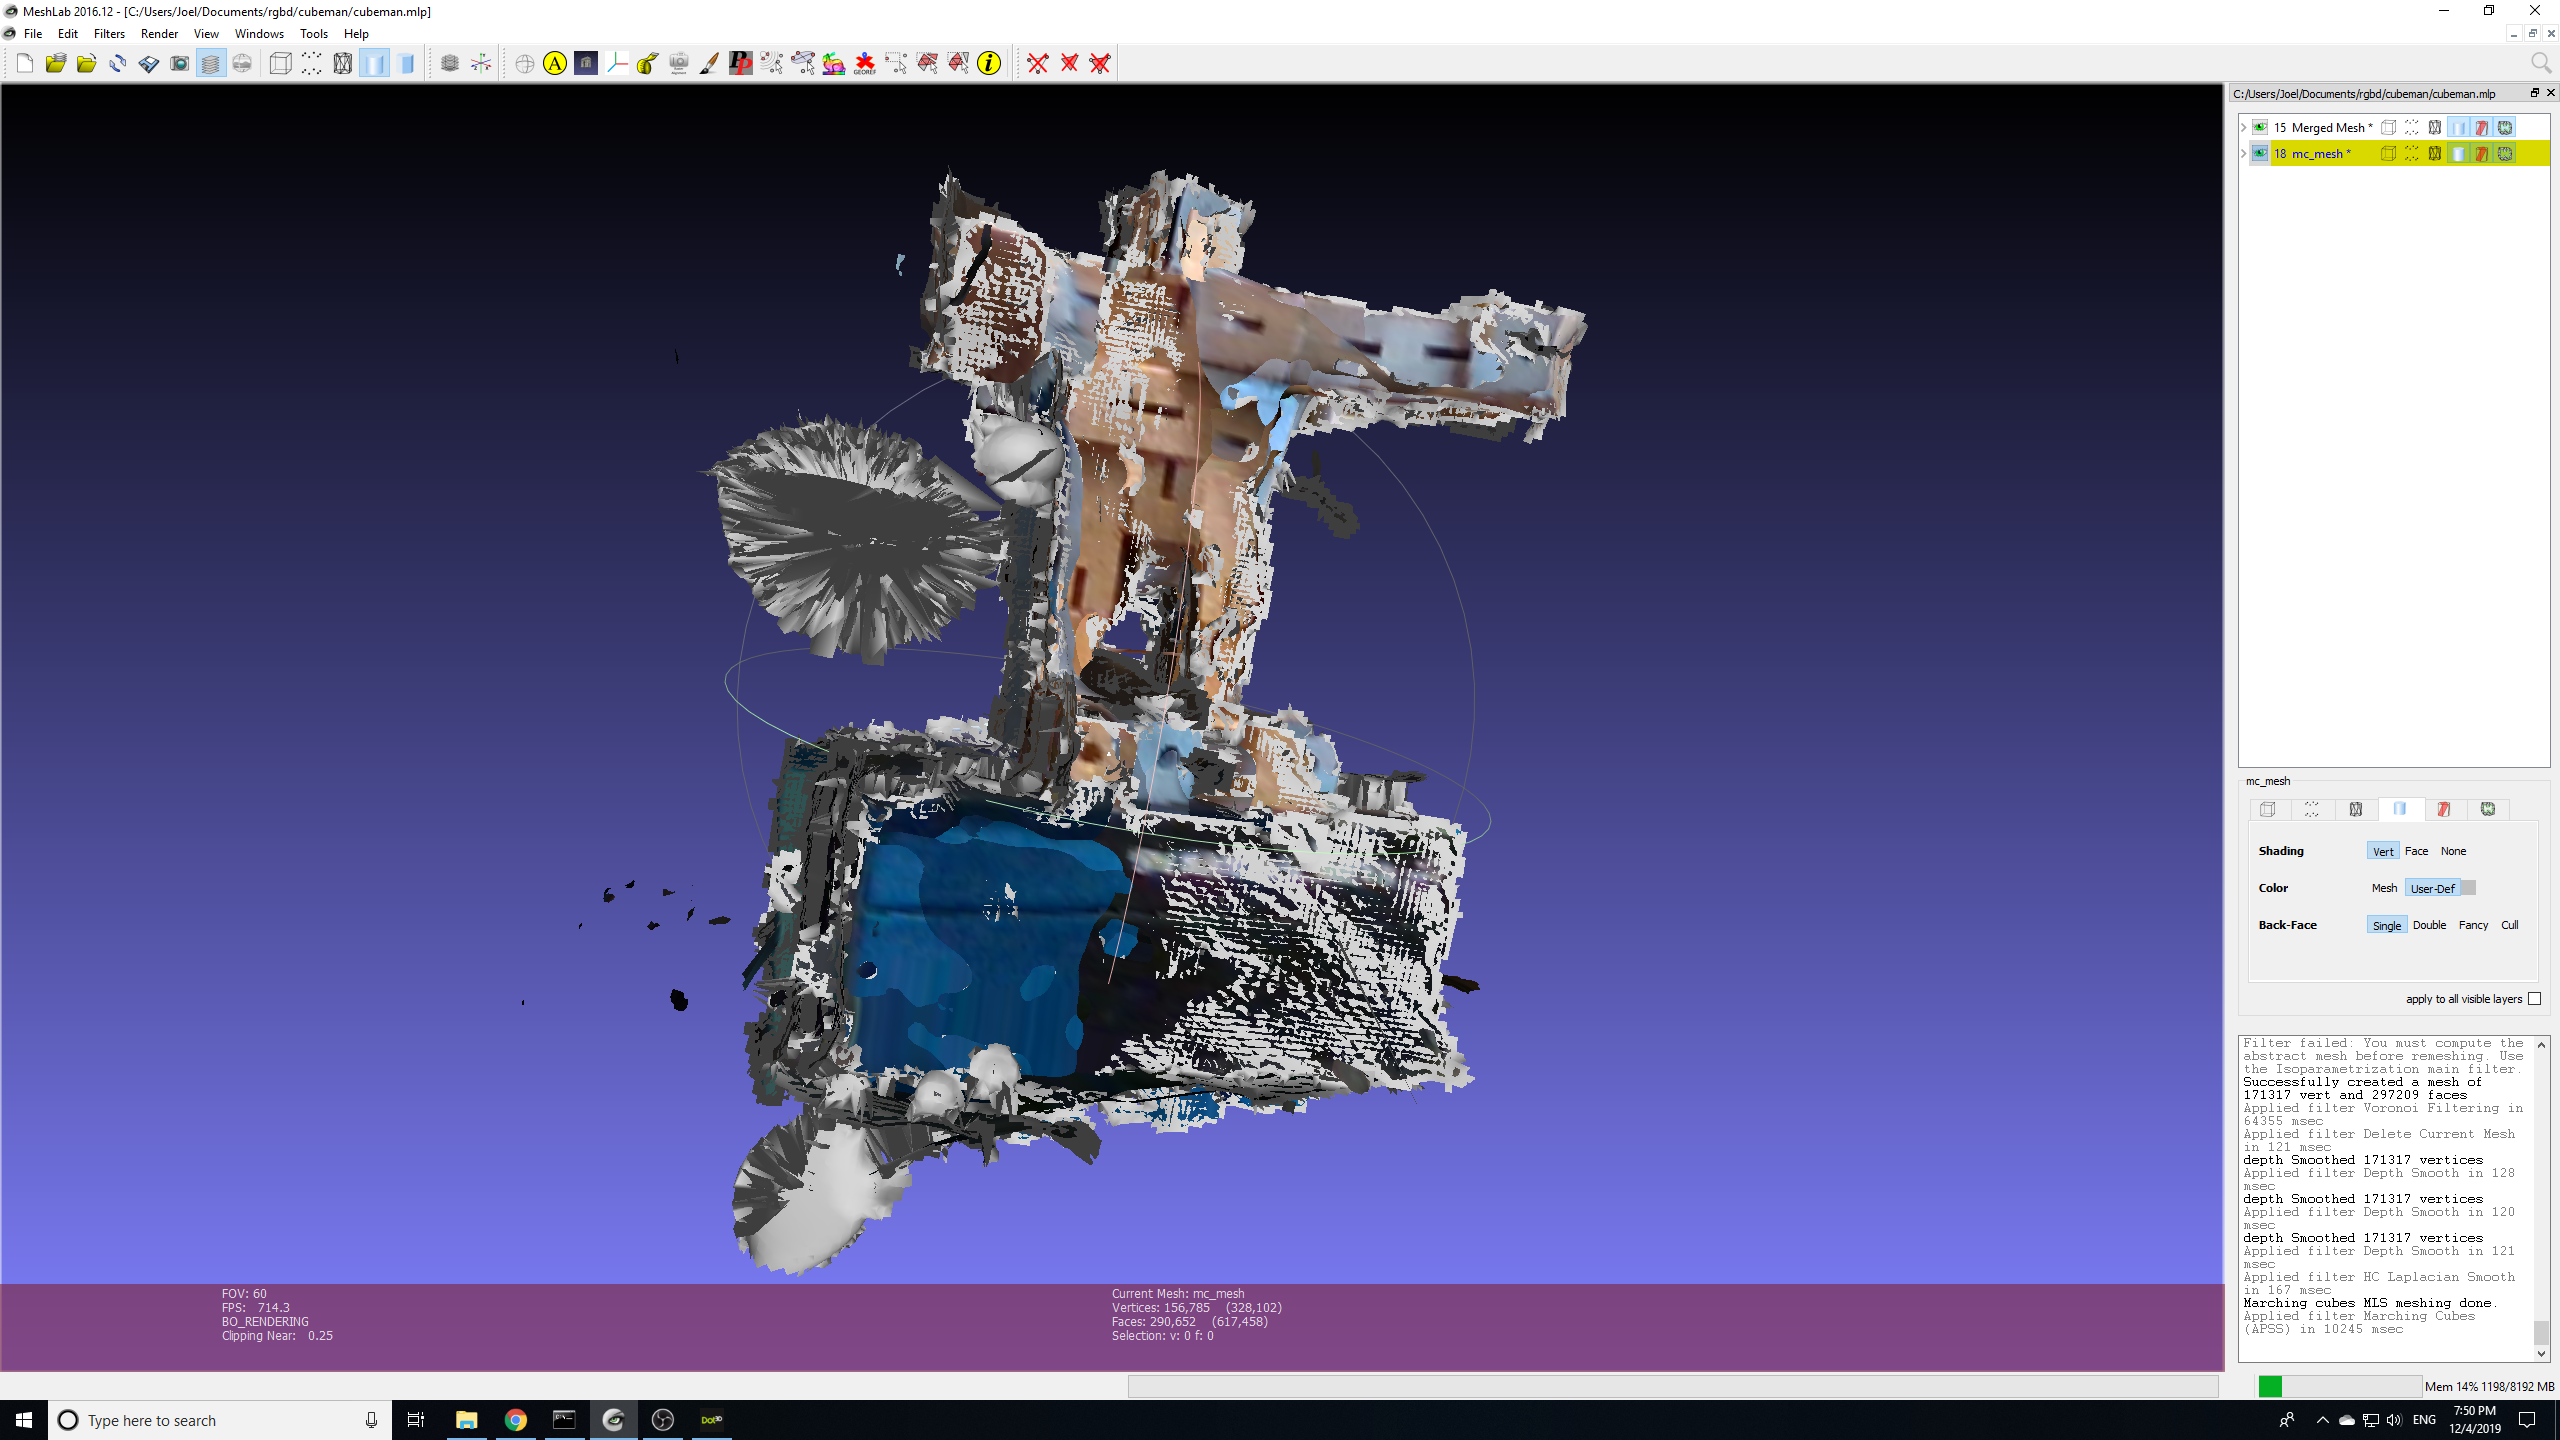
\includegraphics[width=0.6\textwidth]{cube_man_reconstruction1.PNG}
\caption{Reconstruction after first attempt of aligning layers}
\end{figure}

This can be somewhat improved by performing simplification or subsampling operations.
MeshLab offers dozens of filters to perform different operations on meshes, including
these so called mesh ``healing'' filters.

Simple \textit{merge close vertices} collapses vertices within a certain radius
of one another. Another example is \textit{clustering decimation} which similarly detects
and merges neighbourhoods or clusters of points.

\begin{figure}[h]
\centering
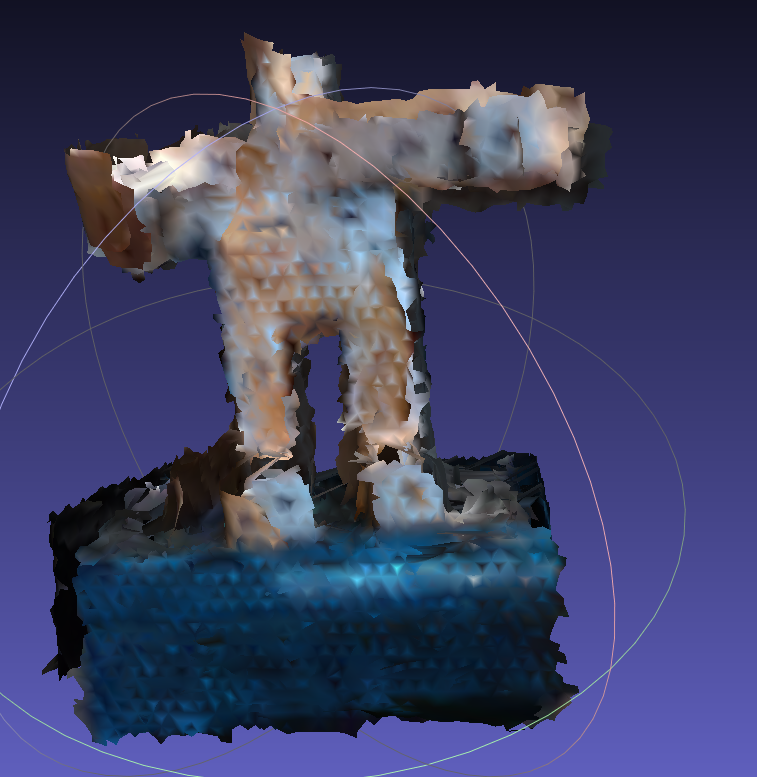
\includegraphics[width=0.6\textwidth]{clustering_decimation.png}
\caption{Simplifying merged cloud with clustering decimation}
\end{figure}

Another possibility is to subsample the points, for example with \textit{poisson sampling}.

\begin{figure}[h]
\centering
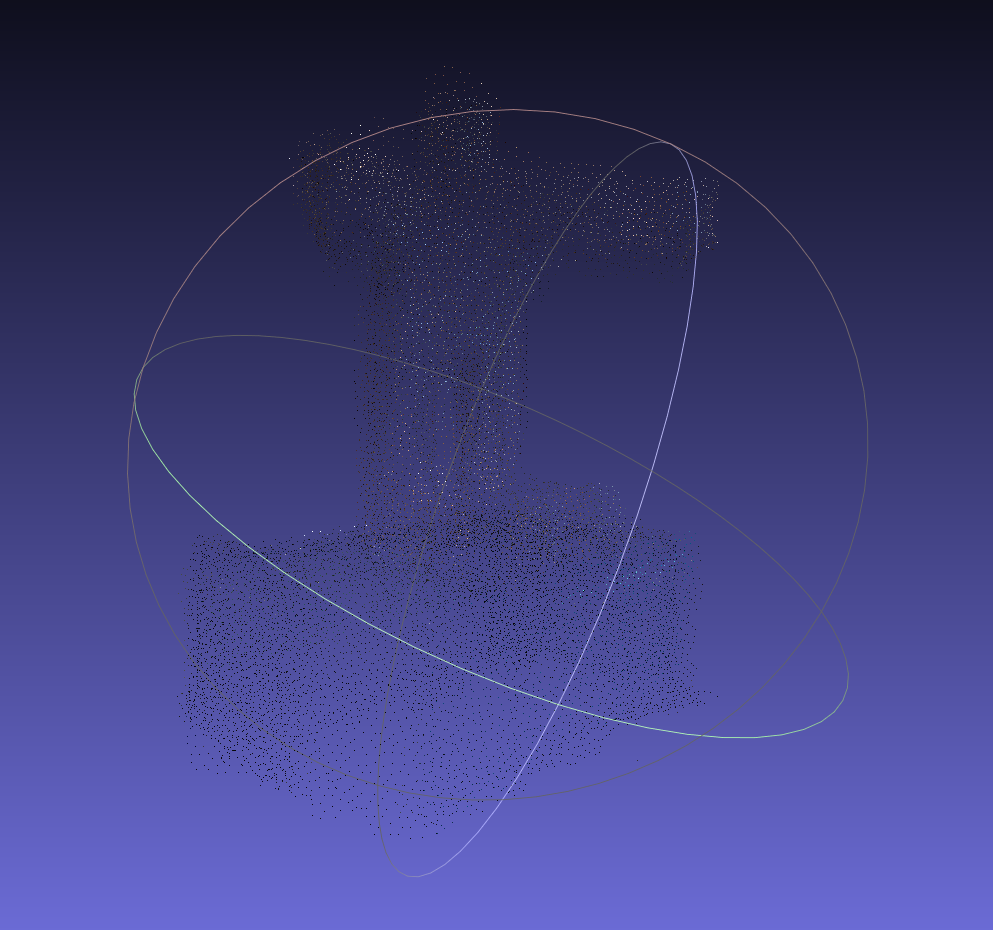
\includegraphics[width=0.6\textwidth]{simplified_point_cloud.png}
\caption{Poisson sampling of merged point point cloud}
\end{figure}

It may also be helpful to \textit{recompute and smooth the normals} after alignment and simplification:
the additional vertices might improve the estimates generated by the camera.

\begin{figure}[H]
\centering
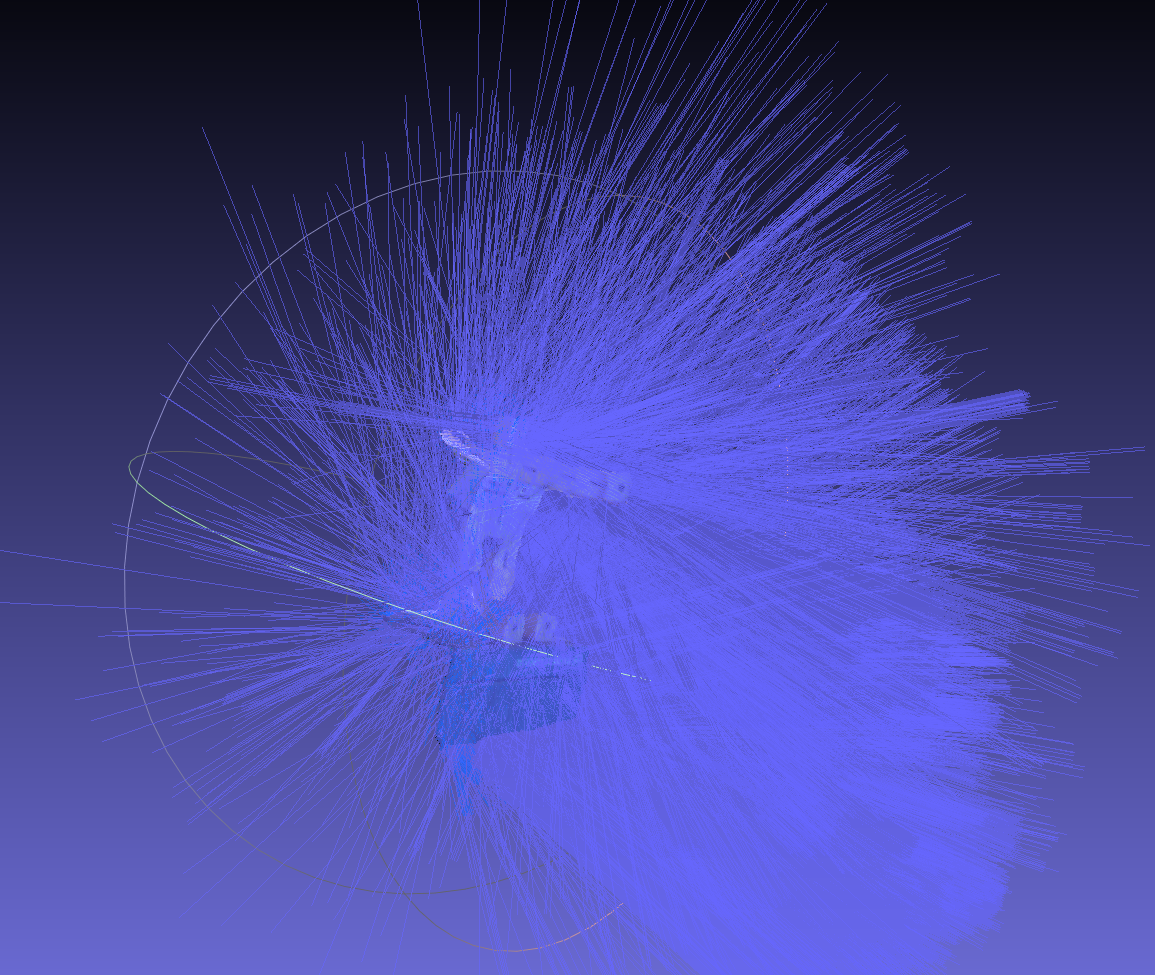
\includegraphics[width=0.4\textwidth]{provided_normals.png}
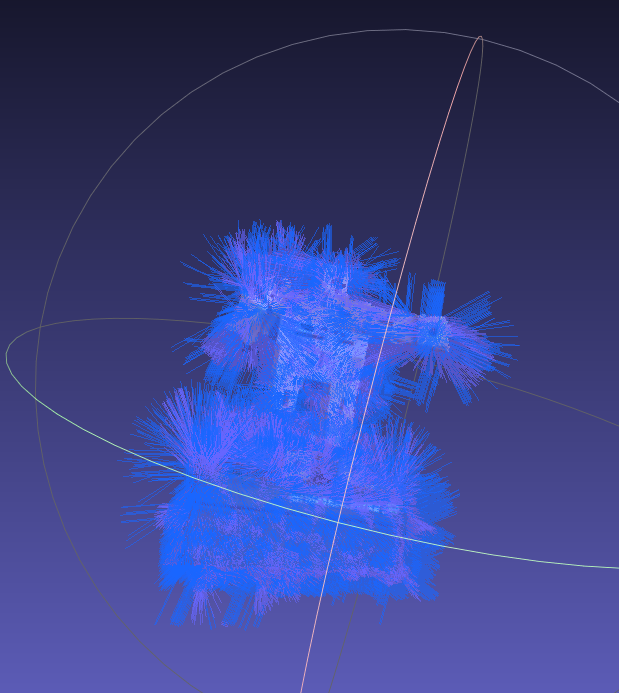
\includegraphics[width=0.4\textwidth]{normals_after_recalculation_filter_and_smoothing.png}
\caption{Normals as generated by Camera and Viewer (left) and after normal smoothing (right)}
\end{figure}
